\documentclass[11pt,a4paper]{article}
\usepackage[margin=2.1cm]{geometry}
\usepackage{booktabs}
\usepackage{tabularx}
\usepackage{longtable}
\usepackage{array}
\usepackage{tikz}
\usepackage{tikz-timing}
\usetikzlibrary{positioning,arrows.meta,fit,automata}
\usepackage{xcolor}
\usepackage{enumitem}
\usepackage{listings}
\usepackage{caption}
\usepackage{bytefield}
\usepackage[hidelinks]{hyperref}
\usepackage{fancyhdr}

\definecolor{codebg}{HTML}{F4F7F6}
\definecolor{rxc}{HTML}{E6F1FB}
\definecolor{txc}{HTML}{FDF0E3}
\definecolor{outc}{HTML}{EAF5EA}
\newcommand{\sig}[1]{\texttt{#1}}
\newcolumntype{L}{>{\raggedright\arraybackslash}X}
\setlist{itemsep=2pt,topsep=4pt}
\setlength{\parskip}{4pt}
\setlength{\parindent}{0pt}
\lstset{basicstyle=\ttfamily\small,backgroundcolor=\color{codebg},frame=none,xleftmargin=6pt,xrightmargin=6pt,aboveskip=6pt,belowskip=6pt,columns=fullflexible,keepspaces=true,showstringspaces=false}
\tikzset{timing/d/text/.style={font=\scriptsize},timing/rowdist=2.6ex}

\pagestyle{fancy}
\fancyhf{}
\lhead{\small Paul Vincent Bezzina \textbar{} ProEm - Open Source Protocol Emulator}
\rhead{\small Line codec reference}
\cfoot{\small\thepage}

\title{ProEm: The Line Codec\\\large \sig{src/core/line\_codec.sv}}
\author{Paul Vincent Bezzina}
\date{11 October 2026}

\begin{document}
\maketitle
\thispagestyle{fancy}

\begin{abstract}
The line codec is the part of each ProEm channel that touches the wire. On the way in it turns pin levels into bits and a bit clock (\sig{tick}) for the frame chain; on the way out it turns the chain's entries into pin levels, with the right line code, timing, stuffing, start and stop conditions, and output drive. It is the one module where every standard's physical details meet, which is why it is the hardest to read. This document walks through it signal by signal: configuration, the receive path, the transmit state machine, the output stage, and the checks it reports. Names in \sig{typewriter} are the signal names in the RTL, so the text can be read next to the code.
\end{abstract}

\tableofcontents
\newpage

%=====================================================================
\section{Where the codec sits}

Each of the two channels has one codec, between the chip's pins and the channel's frame chain.

\begin{center}
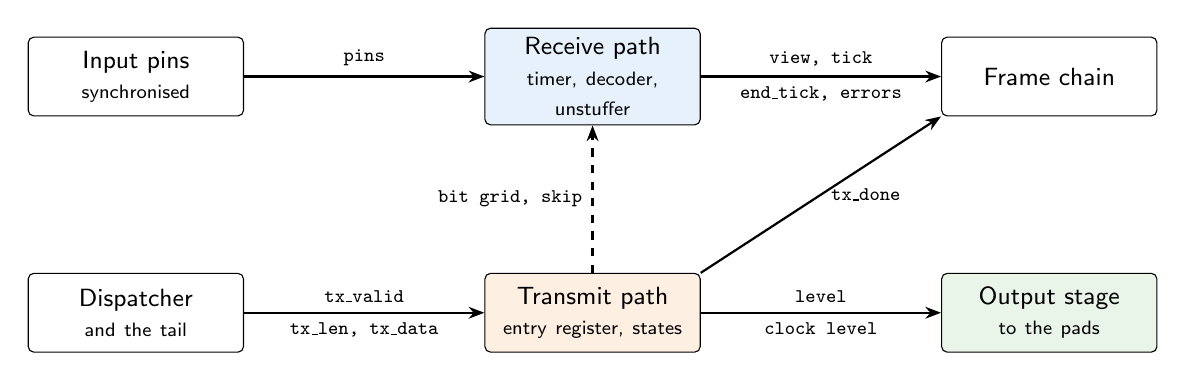
\begin{tikzpicture}[
  box/.style={draw,rounded corners=2pt,align=center,font=\small\sffamily,minimum height=1cm,text width=2.5cm},
  arr/.style={-{Stealth[length=2mm]},thick},
  lab/.style={font=\scriptsize\ttfamily,align=center}]
\node[box] (pins) at (0,2) {Input pins\\\scriptsize synchronised};
\node[box,fill=rxc] (rx) at (5.8,2) {Receive path\\\scriptsize timer, decoder, unstuffer};
\node[box] (chain) at (11.6,2) {Frame chain};
\node[box] (disp) at (0,-1) {Dispatcher\\\scriptsize and the tail};
\node[box,fill=txc] (tx) at (5.8,-1) {Transmit path\\\scriptsize entry register, states};
\node[box,fill=outc] (out) at (11.6,-1) {Output stage\\\scriptsize to the pads};
\draw[arr] (pins) -- node[lab,above]{pins} (rx);
\draw[arr] (rx) -- node[lab,above]{view, tick} node[lab,below]{end\_tick, errors} (chain);
\draw[arr] (disp) -- node[lab,above]{tx\_valid} node[lab,below]{tx\_len, tx\_data} (tx);
\draw[arr] (tx) -- node[lab,above]{level} node[lab,below]{clock level} (out);
\draw[arr] (tx.north east) ++(0,0) -- node[lab,right,pos=0.5]{tx\_done} (chain.south west);
\draw[arr,dashed] (tx.north) -- node[lab,left]{bit grid, skip} (rx.south);
\end{tikzpicture}
\end{center}

\begin{itemize}
\item \textbf{Receive.} Every input pin has already passed through two synchroniser flip-flops and one more register in \sig{protocol\_emulator}, so the codec sees clean, three-clock-late copies of the pads. It produces the pins the chain reads (\sig{view}), one \sig{tick} per bit, a second strobe for END (\sig{end\_tick}), and error and I\textsuperscript{2}C condition flags.
\item \textbf{Transmit.} The dispatcher (and, since v0.6, the chain's tail for the CRC and reply) hands over \emph{wire entries} of 0 to 8 bits. The codec holds one waiting entry, shifts bits out, and reports \sig{tx\_done} after each entry.
\item \textbf{The two halves talk.} The transmitter uses the receive timer to align the reply gap, and the receiver resets its stuffing count when a transmission starts and ignores its own stuff errors while sending.
\end{itemize}

%=====================================================================
\section{Ports}

\begin{longtable}{@{}l l p{8.4cm}@{}}
\toprule
Port & Dir & Meaning \\
\midrule
\endhead
\sig{pins[7:0]} & in & The eight protocol pads, synchronised. \\
\sig{line\_config[15:0]} & in & \sig{LINE} instruction: code, inversion, pins, stuffing. \\
\sig{clock\_config[31:0]} & in & \sig{CLOCK} instruction: tick source, edges, idle level, clock pin, \sig{end\_tick} select, divider. \\
\sig{out\_config[7:0]} & in & \sig{OUT} instruction: drive mode, idle level, pair, end of packet, I\textsuperscript{2}C, select polarity. \\
\sig{listen} & in & A read block wants a bit. With a generated clock this makes the codec run one clock period. \\
\sig{line\_free} & in & Every written bit of the frame has left the codec. Used for stuffing and the select output. \\
\sig{in\_frame} & in & The frame's START has matched or been sent. Unstuffing only arms inside a frame. \\
\sig{frame\_mark} & in & The frame's status entry reached the dispatcher: every bit of the frame has been handed over. Triggers STOP or the end of packet. \\
\sig{halt} & in & \sig{HALT} instruction; ends the current packet like a frame mark. \\
\sig{tx\_cancel} & in & Abort: drop the current and waiting entries and release the line. \\
\sig{tx\_valid}, \sig{tx\_len[3:0]}, \sig{tx\_data[7:0]} & in & A wire entry offered by the dispatcher or the tail. \\
\midrule
\sig{tx\_ready} & out & The waiting-entry register is empty and no end of frame is pending. \\
\sig{tx\_done} & out & One pulse per entry finished (sent, skipped, waited or dropped). \\
\sig{view[7:0]} & out & The pins as the chain sees them: \sig{PIN\_A} replaced by the decoded bit on a timed line. \\
\sig{tick} & out & One pulse per bit for the chain's blocks. \\
\sig{end\_tick} & out & Strobe for the END block, selected by \sig{ETK}. \\
\sig{code\_error} & out & A stuff bit had the wrong value (aborts the frame with a line error). \\
\sig{strict\_tx} & out & The line has fixed timing (not a generated clock), so running out of data is an underrun. \\
\sig{tx\_mismatch} & out & The pad read back differently from what the codec drove (arbitration). \\
\sig{i2c\_target}, \sig{i2c\_start}, \sig{i2c\_stop} & out & I\textsuperscript{2}C target mode is on; START or STOP seen on the bus. \\
\sig{data\_out}, \sig{data\_oe} & out & Data output and its enable. \\
\sig{pair\_out}, \sig{pair\_oe} & out & Complement output (USB D$-$) and its enable. \\
\sig{clock\_out}, \sig{clock\_oe} & out & Generated clock and its enable. \\
\sig{select\_out} & out & Chip select, active from START until the last bit has gone. \\
\bottomrule
\end{longtable}

%=====================================================================
\section{Configuration and derived signals}

The three configuration words are registers in the control unit, written by \sig{LINE}, \sig{CLOCK} and \sig{OUT}. The codec only slices them.

\begin{center}\small
\begin{tabularx}{\linewidth}{@{}l l l L@{}}
\toprule
Word & Bits & RTL name & Instruction field \\
\midrule
\sig{line\_config} & 15:13 & \sig{code} & \sig{LINE} \sig{CODE}: 0 NRZ, 1 NRZI, 2 NRZI pair, 3 Manchester, 4 Manchester Thomas \\
 & 12 & \sig{inv} & \sig{INV} \\
 & 11 & \sig{boundary} & \sig{BND}: Manchester, first edge after idle is a bit boundary (v0.7) \\
 & 10:8 & \sig{pinA} & \sig{PIN\_A}, the data pin \\
 & 7 & \sig{stuffAny} & \sig{SANY}: stuffing counts runs of either value \\
 & 6:3 & \sig{stuffLen} & \sig{STUFF}: run length, 0 = off \\
 & 2:0 & \sig{pinB} & \sig{PIN\_B}, second wire of a pair \\
\midrule
\sig{clock\_config} & 31:30 & \sig{source} & \sig{SRC}: 0 SYNC, 1 ASYNC, 2 GENERATE, 3 RECOVER \\
 & 29:28 & \sig{edgeSel} & \sig{EDGE}: 0 rising, 1 falling, 2 both \\
 & 27 & \sig{clockIdle} & \sig{IDLE}: generated clock level between frames \\
 & 26:24 & \sig{clockPin} & \sig{PIN}: clock input, or the read-back of a generated clock \\
 & 23:22 & \sig{endSel} & \sig{ETK}: what \sig{end\_tick} is \\
 & 21:16, 15:0 & \sig{div} & \sig{DIV}, 22 bits (v0.7): clocks per bit (timed) or per half period (generated) \\
\midrule
\sig{out\_config} & 7:6 & \sig{drive} & \sig{DRIVE}: 0 off, 1 push-pull while sending, 2 open drain, 3 push-pull always \\
 & 5 & \sig{outIdle} & \sig{IDLE}: data level between frames \\
 & 4 & \sig{pairEnable} & \sig{PAIR}: drive the complement output \\
 & 3 & \sig{eopEnable} & \sig{EOP}: end of packet at the end of each frame \\
 & 2 & \sig{i2c} & \sig{I2C}: I\textsuperscript{2}C conditions \\
 & 1 & \sig{selectHigh} & \sig{CSH}: select output active high \\
\bottomrule
\end{tabularx}
\end{center}

From these the codec derives a set of one-bit modes that the rest of the logic uses instead of the raw fields:

\begin{center}
\begin{tabularx}{\linewidth}{@{}l l L@{}}
\toprule
Signal & Definition & Meaning \\
\midrule
\sig{timed} & \sig{source} = ASYNC or RECOVER & The codec's own bit timer sets the bit grid. \\
\sig{generating} & \sig{source} = GENERATE & The codec drives the clock output. \\
\sig{manchester} & \sig{code} = 3 or 4 & Manchester decode and encode. \\
\sig{thomas} & \sig{code} = 4 & Opposite Manchester convention. \\
\sig{nrzi} & \sig{code} = 1 or 2 & NRZI: no change is 1, change is 0. \\
\sig{pairCode} & \sig{code} = 2 & NRZI on a differential pair; SE0 and SE1 detected. \\
\sig{openDrain} & \sig{drive} = 2 & Drive low for 0, release for 1, on data and clock. \\
\sig{i2cTarget} & \sig{i2c} and \sig{source} = SYNC & I\textsuperscript{2}C target: SCL is an input. \\
\sig{half} & \sig{div} $\gg$ 1 & Half a bit. All the timers are 22 bits wide, like \sig{div}, so the slowest bit is 4\,194\,303 clocks (84\,ms at 50\,MHz). \\
\sig{blank} & $\lfloor 3\,\sig{div} / 4 \rfloor$ & Manchester edge blanking window. \\
\sig{twoBits} & 2 $\times$ \sig{div} & Manchester lock timeout, and the length of the end of packet. \\
\bottomrule
\end{tabularx}
\end{center}

%=====================================================================
\section{Receive path}

\subsection{Pin selection}

\begin{lstlisting}
rawA    = pins[pinA]           the data pad as it is
lineA   = rawA ^ inv           the data line in "logical" polarity
lineB   = pins[pinB]           second wire of a pair (USB D-)
clockIn = pins[clockPin]       the clock pad (SYNC input, or GENERATE read-back)
\end{lstlisting}

Each signal also has a one-clock-old copy (\sig{prevA}, \sig{prevRaw}, \sig{prevClock}), which gives the edge detectors: \sig{aEdge} (any change of \sig{lineA}), \sig{clockRise}, \sig{clockFall}. On a pair, \sig{se0} is both wires low and \sig{se1} both high. Note that the SE0 and SE1 tests use \sig{rawA}, not \sig{lineA}: they are about the physical wires, whatever the polarity.

\subsection{The three tick sources}

The chain's blocks take one bit per \sig{tick}. Where the tick comes from is the single biggest switch in the codec:

\begin{center}
\begin{tabularx}{\linewidth}{@{}l l L@{}}
\toprule
Source & \sig{tick} = & How \\
\midrule
SYNC & \sig{syncTick} & An edge of \sig{clockIn}: rising, falling or both (\sig{edgeSel} 0, 1, 2). The chain reads the raw pins on that edge. Used for SPI target, PS/2, I\textsuperscript{2}C target, a looped-back clock. \\
ASYNC, RECOVER & \sig{rxTick} & The receive bit timer below: one tick per decoded, non-stuff bit, with the decoded bit placed on \sig{PIN\_A} of \sig{view}. Used for UART, USB, CAN, Manchester. \\
GENERATE & \sig{genTick} & The transmit state machine, on the sampling edge of the clock it is generating (Section~\ref{sec:gen}). Used for SPI controller and I\textsuperscript{2}C controller. \\
\bottomrule
\end{tabularx}
\end{center}

\sig{view} is the raw \sig{pins} except on a timed line, where \sig{view[pinA]} is replaced by \sig{rxBit}, the last decoded bit. END normally reads another pin or uses the pair compare, so it still sees the real line; \sig{end\_tick} gives it a strobe of its own: \sig{endSel} 0 is the same as \sig{tick}, 1 is every system clock, and 2 is \sig{rxStrobe}, the mid-bit sample strobe, which keeps running through stuff bits and SE0 (USB needs that to count two bit times of SE0).

\subsection{The bit timer (NRZ and NRZI)}

For a timed, non-Manchester line, \sig{rxCount} is a counter that measures position inside the current bit:

\begin{lstlisting}
on any edge of lineA       rxCount <= 1         (re-centre)
else if rxCount >= div-1   rxCount <= 0         (next bit boundary)
else                       rxCount <= rxCount + 1
strobe = (rxCount == half)                      (sample in the middle)
\end{lstlisting}

An edge always marks a bit boundary, so the timer restarts there, and the sample is taken half a bit later. Between edges (a run of equal bits) the timer free-runs one bit per \sig{div} clocks. This is the same trick a UART receiver uses, applied to every bit instead of only the start bit, so the receiver follows a sender whose clock is a few percent off for as long as edges keep coming. Bit stuffing exists precisely to guarantee those edges.

\begin{center}
\begin{tikztimingtable}[timing/slope=0.1,xscale=0.62,yscale=1.1]
\sig{lineA} & 3H 16L 32H 6L \\
\sig{rxCount} & 3D{} 16D{1 \dots{} 15, 0} 16D{1 \dots{} 15, 0} 16D{1 \dots{} 15, 0} 6D{1 \dots} \\
\sig{strobe} & 11L G 16L G 16L G 14L \\
\end{tikztimingtable}
\captionof{figure}{Bit timer with \sig{div} = 16: the edge restarts the count, each strobe is 8 clocks after a boundary.}
\end{center}

\subsection{The Manchester decoder}

A Manchester bit always has an edge in its middle, and has an extra edge at its boundary when two equal bits follow each other. The decoder must use the middle edges and ignore the boundary ones. It does that with a blanking window instead of a sample point:

\begin{lstlisting}
strobe = aEdge && (locked ? rxCount > blank : !boundary)     blank = 3/4 of a bit
on strobe:   rxCount <= 1, locked <= 1
first edge after idle with BND set:  rxCount <= half, locked <= 1, no bit
otherwise:   rxCount counts up (saturating); locked <= 0 after two bit times
bit value  = lineA ^ thomas                         the level after the edge
\end{lstlisting}

After an accepted (middle) edge, any edge within $\frac34$ of a bit is a boundary edge and is ignored; the next middle edge comes one bit later, well past the window. If the line goes quiet for two bit times, \sig{locked} drops and the next edge is accepted at once, which is how the decoder catches the first edge of a frame. With IEEE convention a low-to-high middle edge is a 1, so the level after the edge is the bit; Thomas convention inverts it.

\paragraph{The first edge after idle (v0.7).} Taking the first edge as a middle edge is right when a frame begins with a preamble (10BASE-T) or with a bit whose first half equals the idle level (RC5). It is wrong when the first bit's first half differs from idle, as in DALI, whose start bit falls from the idle-high bus at the bit boundary: the decoder would then lock half a bit out of phase. With \sig{BND} set, the first edge after idle produces no bit; it sets \sig{rxCount} to half a bit and \sig{locked}, so the middle edge half a bit later sees \sig{rxCount} at a full bit, passes the window, and is decoded as the first bit. One edge after idle cannot tell the two cases apart by timing alone, because a boundary edge also follows a middle edge whenever two equal bits are sent, which is why this is a setting rather than automatic.

The window must sit strictly between half a bit (a boundary edge) and one bit (the next middle edge), with room for jitter. At 4 clocks per bit, $\frac34$ is 3 clocks and a boundary edge 2 clocks after a middle edge is too close to call once jitter is added, so 5 clocks per bit is the minimum (10BASE-T at 50\,MHz).

\subsection{Bit value per line code}

\begin{center}
\begin{tabularx}{\linewidth}{@{}l l L@{}}
\toprule
Code & \sig{bitValue} & Notes \\
\midrule
NRZ & \sig{lineA} & The sampled level. \\
NRZI, NRZI pair & \sig{lineA == lastSample} & Same level as the last sample is a 1, a change is a 0. \sig{lastSample} is updated on every strobe, and forced to 0 during SE0 or SE1 so the first bit after an end of packet is measured from J. \\
Manchester & \sig{lineA \^{} thomas} & Level after the accepted middle edge. \\
\bottomrule
\end{tabularx}
\end{center}

\sig{dataValid} is a strobe that is not SE0 or SE1: on a pair, those states carry no data bits. They still produce \sig{rxStrobe}, for END.

\subsection{The unstuffer}

When \sig{stuffLen} is not zero, the transmitter has inserted one extra bit after every run of \sig{stuffLen} equal bits, and the receiver must take it out again without giving it a tick. Two styles exist:

\begin{center}
\begin{tabularx}{\linewidth}{@{}l l l L@{}}
\toprule
Standard & \sig{stuffLen} & \sig{stuffAny} & What counts as a run \\
\midrule
USB & 6 & 0 & Consecutive 1s only. The stuff bit is a 0 (in NRZI, a forced transition). \\
CAN & 5 & 1 & Consecutive equal bits, 0s or 1s. The stuff bit is the opposite value. \\
\bottomrule
\end{tabularx}
\end{center}

The state is three registers: \sig{runCount} (length of the current run), \sig{runValue} (its value, for \sig{stuffAny}) and \sig{skipNext} (the next data bit is a stuff bit).

\begin{lstlisting}
runMatch = stuffAny ? (bitValue == runValue) : bitValue
nextRun  = runMatch ? runCount + 1 : (stuffAny ? 1 : 0)

dropBit  = dataValid && stuffOn && skipNext         this bit is a stuff bit
goodBit  = dataValid && !dropBit                    this bit goes to the chain
stuffBad = dropBit && (stuffAny ? bitValue == runValue : bitValue)
\end{lstlisting}

\begin{itemize}
\item On a good bit, the run is extended or restarted, and \sig{skipNext} is set when the run reaches \sig{stuffLen}.
\item On a dropped bit, \sig{skipNext} clears and a new run starts: with \sig{stuffAny} the stuff bit itself is the first bit of the next run (CAN counts it), without it the count restarts at 0 (USB's stuff bit is a 0 and so ends a run of 1s).
\item A stuff bit with the wrong value (\sig{stuffBad}) is registered as \sig{code\_error}, which aborts the frame with a line error. USB uses this as an error check; CAN calls it a stuff error.
\item The run is cleared on SE0 or SE1 (USB end of packet) and when a transmission starts (\sig{txBegin}), so a packet never inherits a run from before it.
\end{itemize}

Three conditions guard \sig{skipNext} and \sig{code\_error}. They were each added after a test failed, so they are worth knowing:

\begin{enumerate}
\item \textbf{Arm only inside a frame} (\sig{in\_frame}). A CAN bus idles recessive (1). Without this, five idle 1s armed the skip and the start-of-frame 0 was thrown away as a stuff bit.
\item \textbf{Arm only when the codec is sending a packet or nothing is queued} (\sig{packetActive || line\_free}). In a transmit frame, \sig{in\_frame} goes high as soon as START is queued, before the first bit is on the wire; idle bits seen in that gap must not count.
\item \textbf{Ignore stuff errors while sending} (\sig{!packetActive}). When the codec is driving a line whose pad is not read back on \sig{PIN\_A}, the decoder sees a static line and would report errors in the chip's own transmission.
\end{enumerate}

\subsection{What the chain receives}

\sig{rxBit} and \sig{rxTick} are registered from \sig{bitValue} and \sig{goodBit}, so the chain sees each bit one clock after its strobe, and the bit and its tick arrive together. A stuff bit produces neither. The chain's CRC unit is fed from the same tick, which is why the CRC never includes stuff bits.

%=====================================================================
\section{Transmit path}

\subsection{Entries in, \sig{tx\_done} out}

The codec holds at most one waiting entry, in \sig{nextValid}, \sig{nextLen} and \sig{nextData}, plus the one it is shifting out (\sig{shiftData}, \sig{shiftLeft}). It accepts a new one whenever the waiting slot is empty:

\begin{lstlisting}
tx_ready = !nextValid && !endPending && !tx_cancel
\end{lstlisting}

Bits leave from bit 0 upward. MSB-first standards are handled by the chain, which reverses each field before it reaches the codec, so the codec never needs to know the bit order. An entry's length is 1 to 8 bits; length 0 is special:

\begin{center}
\begin{tabularx}{\linewidth}{@{}l l L@{}}
\toprule
Entry & Condition & Meaning \\
\midrule
length 0, \sig{data[7]} = 1 & timed, not Manchester & Wait \sig{data[6:0]} bit times without driving, aligned to the receive bit grid (\sig{T\_WAIT}). Used for the reply gap. \\
length 0 & I\textsuperscript{2}C controller, bus busy & Repeated START (\sig{T\_REPEAT}). \\
length 0 & otherwise & Nothing to send; counts as done at once. \\
\bottomrule
\end{tabularx}
\end{center}

Every entry ends with exactly one \sig{tx\_done} pulse, whether it was sent, waited, skipped or dropped by a cancel. The chain counts entries in flight with it and only lets read blocks listen once that count is zero (\sig{line\_free}).

\sig{endPending} is set by \sig{frame\_mark} or \sig{halt}. It stops new entries being taken until the end-of-frame action (STOP or end of packet) has been done, so the next frame's bits can never slip in before it.

\subsection{The state machine}

\begin{center}
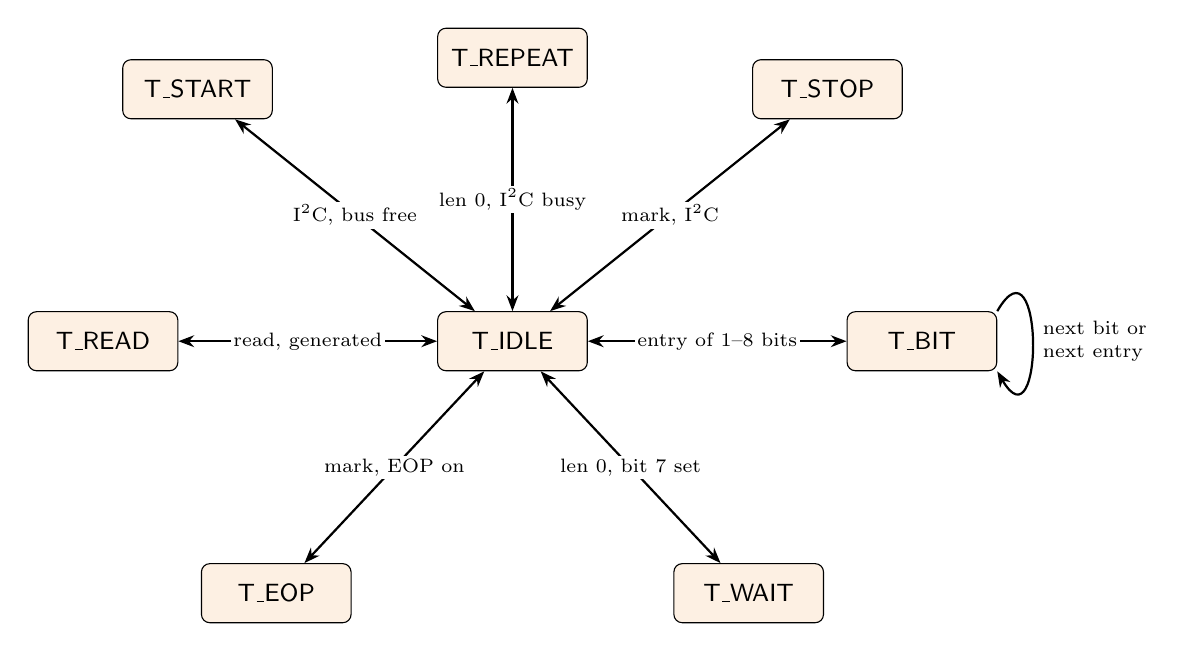
\begin{tikzpicture}[
  st/.style={draw,rounded corners=3pt,minimum width=1.9cm,minimum height=0.75cm,font=\small\sffamily,fill=txc},
  arr/.style={{Stealth[length=2mm]}-{Stealth[length=2mm]},thick},
  lab/.style={font=\scriptsize,align=center,fill=white,inner sep=1pt}]
\node[st] (idle) at (0,0) {T\_IDLE};
\node[st] (bit) at (5.2,0) {T\_BIT};
\node[st] (read) at (-5.2,0) {T\_READ};
\node[st] (start) at (-4,3.2) {T\_START};
\node[st] (rep) at (0,3.6) {T\_REPEAT};
\node[st] (stop) at (4,3.2) {T\_STOP};
\node[st] (eop) at (-3,-3.2) {T\_EOP};
\node[st] (wait) at (3,-3.2) {T\_WAIT};
\draw[arr] (idle) -- node[lab]{entry of 1--8 bits} (bit);
\draw[arr] (idle) -- node[lab]{read, generated} (read);
\draw[arr] (idle) -- node[lab]{I\textsuperscript{2}C, bus free} (start);
\draw[arr] (idle) -- node[lab]{len 0, I\textsuperscript{2}C busy} (rep);
\draw[arr] (idle) -- node[lab]{mark, I\textsuperscript{2}C} (stop);
\draw[arr] (idle) -- node[lab]{mark, EOP on} (eop);
\draw[arr] (idle) -- node[lab]{len 0, bit 7 set} (wait);
\draw[-{Stealth[length=2mm]},thick] (bit.north east) to[out=60,in=-60,looseness=4] node[font=\scriptsize,right,align=left]{next bit or\\next entry} (bit.south east);
\end{tikzpicture}
\end{center}
Every state returns to \sig{T\_IDLE} when it is done; \sig{T\_BIT} stays as long as bits, stuff bits or a waiting entry keep coming.

\sig{T\_IDLE} decides what to do next, in this order of priority:

\begin{enumerate}
\item A waiting length-0 entry: start a wait, a repeated START, or simply finish it.
\item A waiting entry on an idle I\textsuperscript{2}C controller bus: send START first (\sig{T\_START}); the entry is sent afterwards.
\item A waiting entry, and (I\textsuperscript{2}C target only) SCL has just fallen: load it and send (\sig{T\_BIT}). This is \sig{txBegin} when no packet is active.
\item Generated clock, a read block listening, no end pending: run one clock period with the line released (\sig{T\_READ}).
\item An end pending: STOP on an I\textsuperscript{2}C controller (\sig{T\_STOP}), end of packet if enabled (\sig{T\_EOP}), otherwise just close the packet.
\end{enumerate}

A \sig{tx\_cancel} overrides everything: it goes to \sig{T\_IDLE}, clears the packet, I\textsuperscript{2}C and stuffing state, and sets \sig{dropCount} to the number of entries it threw away (the one being shifted, if any, plus the waiting one), so \sig{tx\_done} is still pulsed once for each over the next clocks.

\subsection{Packets}

\sig{packetActive} is set when the first entry of a frame starts and cleared at the end of packet, STOP, or the end-of-frame action. While it is set:
\begin{itemize}
\item the NRZI level and the transmit stuffing run carry on from one entry to the next, so a frame made of many entries is one continuous coded stream;
\item between entries, when the next one has not arrived yet, the line holds the last level sent (\sig{holdLevel}) instead of going to the idle level. An I\textsuperscript{2}C target with open drain is the exception: it releases SDA.
\end{itemize}
When the first entry of a packet loads, the transmit run is cleared and the NRZI level is set as if the line had been at J: \sig{nrziLevel} = \sig{!data[0]}.

\subsection{Bit timing}\label{sec:gen}

\sig{T\_BIT} sends one bit at a time; \sig{txCount} measures time inside the bit, and \sig{endOfBit} says when to move on. It depends on the tick source:

\begin{center}
\begin{tabularx}{\linewidth}{@{}l L@{}}
\toprule
Source & Bit timing \\
\midrule
Timed & One bit every \sig{div} clocks: \sig{endOfBit} at \sig{txCount} = \sig{div} $-$ 1. The transmit grid is free-running and independent of the receive timer. \\
SYNC & The output changes on the clock edge opposite the sampling edge (\sig{shiftEdge}): falling if the chain samples on rising, and rising if it samples on falling. Used for SPI target and I\textsuperscript{2}C target. \\
Generated & Two phases of \sig{div} clocks each. Phase A (\sig{phaseB} = 0) holds the clock at \sig{phaseAClock}, its idle level (forced low for I\textsuperscript{2}C); phase B holds the opposite level. The data changes at the start of phase A, so it is stable across the A-to-B edge. \\
\bottomrule
\end{tabularx}
\end{center}

\paragraph{Generated clock details.}
\begin{itemize}
\item \sig{sampleLeading} says whether the chain samples on the A-to-B edge (the middle of the bit) or on the B-to-A edge (the end). It is true when \sig{edgeSel} is ``both'', or when the chosen edge is the one that leaves the idle level. SPI modes 0 and 3 sample on the leading edge; modes 1 and 2 on the trailing one. \sig{genTick} pulses on the chosen edge, which is how the chain gets its tick in this mode.
\item Clock stretching: in phase B, with open drain, the codec has released the clock and waits until the clock read-back (\sig{clockIn}, the clock pin) is actually high (\sig{clockHigh}) before it starts counting. A slow I\textsuperscript{2}C device holding SCL low therefore just lengthens the bit.
\item The clock only runs while there is something to do: a bit to send (\sig{T\_BIT}) or a read block listening (\sig{T\_READ}). Between bytes on I\textsuperscript{2}C the controller holds SCL low.
\item Where the sample falls. \sig{genTick} is registered and the input pins are three clocks late, so with a push-pull clock the chain sees the line as it was about one system clock before the chip's sampling edge, which suits any device that changes its output on or after that edge (MDIO, SPI). With an open-drain clock the codec first waits for the read-back to show the clock high, so the sample is taken just after the edge; I\textsuperscript{2}C needs this because a target may change SDA while it stretches SCL.
\end{itemize}

\begin{center}
\begin{tikztimingtable}[timing/slope=0.1,xscale=0.9,yscale=1.0]
clock (idle 0) & 2L 4L 4H 4L 4H 2L \\
data & 2H 8D{bit 0} 8D{bit 1} 2H \\
phase & 2D{} 4D{A} 4D{B} 4D{A} 4D{B} 2D{} \\
\sig{genTick} (rising) & 6L G 8L G 6L \\
\end{tikztimingtable}
\captionof{figure}{Generated clock, SPI mode 0: \sig{div} clocks per phase, data set at the start of phase A, sampled on the rising A-to-B edge.}
\end{center}

\subsection{Shifting, stuffing and chaining entries}

At \sig{endOfBit} the machine decides the next bit. The combinational signals computed for that moment are:

\begin{lstlisting}
dataBitEnded = !stuffing                    the bit just sent was data, not a stuff bit
txRunNew     = run length including it      (stuffAny: equal bits; else 1s)
willStuff    = dataBitEnded && stuffOn && txRunNew == stuffLen
stuffValue   = stuffAny ? !sendBit : 0
leftAfter    = shiftLeft - (dataBitEnded ? 1 : 0)
entryDone    = !willStuff && leftAfter == 0
continueNext = entryDone && nextValid && nextLen != 0
nextBitValue = willStuff ? stuffValue : (entryDone ? nextData[0] : dataAfter[0])
\end{lstlisting}

\begin{itemize}
\item A stuff bit is sent \emph{instead of} advancing the shift register: \sig{stuffing} is set, \sig{sendBit} becomes \sig{stuffValue}, and the data stays where it was. After the stuff bit, the run restarts (at 1 with \sig{stuffAny}, since CAN counts the stuff bit; at 0 for USB).
\item An entry is not done while a stuff bit is still owed after its last bit. That is why a CAN CRC that ends in five equal bits is followed by its stuff bit before the delimiter.
\item If the next entry is already waiting when the current one ends, its first bit follows with no gap (\sig{continueNext}). If not, the machine returns to \sig{T\_IDLE}, the line holds its level, and the next entry starts a fresh bit period when it arrives. On a timed line that pause shows up as a longer bit, which is why the chain keeps the codec fed and reports an underrun if it cannot.
\item \sig{tx\_done} pulses when \sig{entryDone}.
\end{itemize}

\subsection{From bit to level}

\begin{center}
\begin{tabularx}{\linewidth}{@{}l L@{}}
\toprule
Code & \sig{bitLevel} \\
\midrule
NRZ & \sig{sendBit}. \\
NRZI & \sig{nrziLevel}, which toggles for every 0 and holds for every 1 (updated together with \sig{sendBit}). \\
Manchester & On a timed line, \sig{!sendBit} for the first half of the bit and \sig{sendBit} for the second (XOR \sig{thomas}), so a 1 is a low-to-high middle edge. \sig{div} must be even. \\
\bottomrule
\end{tabularx}
\end{center}

\sig{level} is then chosen by state (Section~\ref{sec:levels}), and the pad value is \sig{dataPin} = \sig{level \^{} inv}, or 0 during SE0.

\subsection{I\textsuperscript{2}C conditions}

On an I\textsuperscript{2}C controller (generated clock with \sig{i2c}), three states draw the bus conditions, each in steps of \sig{div} clocks. In steps that raise SCL with open drain, the step waits until SCL really is high, so stretching works here too.

\begin{center}
{\small\begin{tabular}{@{}l c c c c l@{}}
\toprule
State & Step 0 & Step 1 & Step 2 & Step 3 & Result \\
\midrule
\sig{T\_START} & SDA 0, SCL 1 & SDA 0, SCL 0 & & & SDA falls while SCL is high \\
\sig{T\_REPEAT} & SDA 1, SCL 0 & SDA 1, SCL 1 & SDA 0, SCL 1 & SDA 0, SCL 0 & repeated START \\
\sig{T\_STOP} & SDA 0, SCL 0 & SDA 0, SCL 1 & SDA 1, SCL 1 & & SDA rises while SCL is high \\
\bottomrule
\end{tabular}}
\end{center}

\sig{i2cBusy} is set after START and cleared after STOP. While it is set, the idle state holds SCL low. As a target (SYNC clock on SCL), the codec does not draw conditions; it detects them:

\begin{lstlisting}
i2c_start = SDA falls (prevRaw && !rawA) while SCL is high now and last clock
i2c_stop  = SDA rises (!prevRaw && rawA) while SCL is high now and last clock
\end{lstlisting}
and waits for SCL to fall (\sig{startWait}) before driving each new bit, so its data meets the bus's hold and set-up rules.

\subsection{End of packet}

When the end is pending, a packet is active and \sig{eop} is set, \sig{T\_EOP} sends:
\begin{itemize}
\item on a pair (USB): two bit times of SE0 (both outputs low, \sig{se0Out}), then one bit time of J, then the line is released;
\item on a single line (10BASE-T): two bit times high.
\end{itemize}
The NRZI level is reset afterwards, so the next packet starts from J again.

\subsection{Waiting on the receive grid}

\sig{T\_WAIT} implements the wait entry used for the reply gap. It does not drive anything (the level is the idle level), and works in two parts:

\begin{enumerate}
\item \textbf{Align.} Wait until the receive timer reaches a bit boundary (\sig{rxCount} $\ge$ \sig{div} $-$ 1). If the unstuffer has a stuff bit pending at that moment (\sig{skipNext}), add one bit to the wait: that bit belongs to the frame just received (CAN after a CRC ending in five equal bits).
\item \textbf{Count.} Count \sig{waitBits} bit times of \sig{div} clocks, then finish the entry.
\end{enumerate}

The reply that follows therefore starts exactly on the bit grid of the frame it answers, which is what a CAN ACK slot demands.

%=====================================================================
\section{Output stage}\label{sec:levels}

\subsection{Line and clock level by state}

\begin{center}
\begin{tabularx}{\linewidth}{@{}l l L@{}}
\toprule
State & \sig{level} (data) & \sig{clockLevel} \\
\midrule
\sig{T\_IDLE}, \sig{T\_WAIT} & \sig{idleLevel} & I\textsuperscript{2}C: low while busy, high when free. Otherwise \sig{clockIdle}. \\
\sig{T\_BIT} & \sig{bitLevel} & phase A: \sig{phaseAClock}; phase B: the opposite \\
\sig{T\_READ} & released (1 open drain, else \sig{outIdle}) & as \sig{T\_BIT} \\
\sig{T\_START}, \sig{T\_REPEAT}, \sig{T\_STOP} & per step (table above) & per step \\
\sig{T\_EOP} & 0 on a pair (SE0, then J), 1 otherwise & \sig{clockIdle} \\
\bottomrule
\end{tabularx}
\end{center}

\sig{idleLevel} is \sig{holdLevel} inside a packet (except an I\textsuperscript{2}C target with open drain), otherwise 1 with open drain or \sig{outIdle} with push-pull.

\subsection{Pads}

\begin{center}
\begin{tabularx}{\linewidth}{@{}l L L@{}}
\toprule
Output & Value & Enable \\
\midrule
data & push-pull: \sig{dataPin}; open drain: 0 & push-pull always (\sig{drive} 3), or while \sig{driveNow} (\sig{drive} 1); open drain: when \sig{dataPin} is 0 \\
pair & \sig{!(level \^{} inv)}, or 0 during SE0 & as push-pull data, if \sig{pair} is set \\
clock & push-pull: \sig{clockLevel}; open drain: 0 & generated clock and \sig{drive} not off; open drain: when \sig{clockLevel} is 0 \\
select & \sig{selectActive}, inverted unless \sig{csH} & no enable (a plain output) \\
\bottomrule
\end{tabularx}
\end{center}

\sig{sending} is any state other than idle and wait, or an active packet. \sig{driveNow} (v0.7) is \sig{sending} except in \sig{T\_READ} and, with a generated clock, in \sig{T\_IDLE}: a ``push-pull while sending'' output lets go of the line for read bits, so a device can answer on the same wire (3-wire SPI, MDIO). Timed lines still hold their level between entries of a packet. \sig{selectActive} covers the whole frame: from START (\sig{in\_frame}) through every queued and in-flight bit (\sig{nextValid}, \sig{!line\_free}), so SPI chip select never glitches between entries. With \sig{drive} = 0, after reset or \sig{CLEAR}, nothing but select is driven.

%=====================================================================
\section{Checks reported to the chain}

\paragraph{Read-back mismatch.} While sending a bit, the codec compares the pad it drives with the pad it reads back on \sig{PIN\_A}, at a \sig{checkPoint}:

\begin{center}
\begin{tabularx}{\linewidth}{@{}l L@{}}
\toprule
Source & Check point \\
\midrule
Timed & middle of the bit (a quarter bit for Manchester, before the middle edge) \\
Generated & middle of phase B, once the clock is high \\
SYNC & the sampling edge \\
\bottomrule
\end{tabularx}
\end{center}

\sig{tx\_mismatch} = \sig{T\_BIT} and check point and \sig{rawA} $\ne$ \sig{dataPin}. The branch unit uses it for CAN-style arbitration: the chip sent recessive and read dominant, so another node won. Because the input pipeline is three clocks long, a timed line needs at least 8 clocks per bit for the check to land inside the bit.

\paragraph{Stuff error.} \sig{code\_error}, described with the unstuffer.

\paragraph{Strict timing.} \sig{strict\_tx} is high for every source except a generated clock: with a generated clock the codec can simply pause, but on a timed or externally clocked line, running out of data mid-frame breaks the frame, so the chain reports an underrun.

%=====================================================================
\section{Worked examples}

\subsection{UART transmit, 115\,200 baud}

\sig{CLOCK} ASYNC, \sig{div} = 434; \sig{LINE} NRZ; \sig{OUT} push-pull always, idle 1. The chain sends a 1-bit entry \{0\} (start bit) from START, then entries of 8 data bits and \{1\} (stop bit) from MAIN. The codec takes the start entry, holds 0 for 434 clocks, chains straight into the data entry (it was already waiting), sends its 8 bits LSB first at 434 clocks each, then the stop bit. At the frame mark there is no end of packet, so the packet just closes and the line returns to \sig{outIdle} = 1.

\subsection{USB low speed receive}

\sig{LINE} NRZI pair, \sig{stuffLen} = 6, \sig{stuffAny} = 0; \sig{CLOCK} RECOVER, \sig{div} = 33. Each edge on D+ restarts \sig{rxCount}; the strobe 16 clocks later samples J or K and compares with the last sample. After six 1s (six bit times without an edge) \sig{skipNext} is set and the next strobe's bit, which must be a 0 (a transition), is dropped without a tick. The two bits of SE0 at the end produce strobes but no data, clear the run, and are counted by END through \sig{end\_tick} = \sig{rxStrobe}.

\subsection{CAN acknowledge}

\sig{LINE} NRZ with \sig{stuffLen} = 5, \sig{stuffAny} = 1; open drain; \sig{CLOCK} ASYNC. As the last CRC bit is sampled, the chain's tail queues a wait entry with \sig{GAP} = 0 and a 2-bit reply \{1, 0\}. \sig{T\_WAIT} waits for the next receive bit boundary, adds one bit if a stuff bit is owed, and finishes. The reply then sends a 1 (released, the CRC delimiter) and a 0 (driven low) exactly in the ACK slot.

\subsection{I\textsuperscript{2}C controller write}

\sig{CLOCK} GENERATE, \sig{div} = 250 (100\,kHz); \sig{OUT} open drain with \sig{i2c}. The first entry finds the bus free: \sig{T\_START} pulls SDA low with SCL high, then SCL low. The address and data bits go out in \sig{T\_BIT}, SDA changing while SCL is low and sampled on the rising edge; the ACK bit is a read, run by \sig{T\_READ} with SDA released. At the frame mark, \sig{T\_STOP} raises SCL and then SDA, and the bus is free again.

%=====================================================================
\section{Limits and rules of thumb}

\begin{itemize}
\item \textbf{Manchester receive} needs at least 5 clocks per bit; \textbf{Manchester transmit} needs an even \sig{div}.
\item \textbf{Generated clocks} need \sig{div} $\ge$ 4 clocks per half period.
\item \textbf{Read-back on a timed line} needs at least 8 clocks per bit (three clocks of input pipeline).
\item \textbf{Seamless transmit} needs the next entry waiting before the current one ends; otherwise the line pauses for at least one clock and a timed bit is stretched.
\item \textbf{The wait entry} needs a timed, non-Manchester line, because it aligns to the receive bit timer; elsewhere it is skipped.
\item \textbf{One data pin per codec.} \sig{PIN\_A} is the only decoded pin; other pins are seen raw.
\item \textbf{Bit rate range.} With the 22-bit \sig{div}, from 12\,bit/s up to the per-code minimums above, at 50\,MHz.
\end{itemize}

%=====================================================================
\section{How it is tested}

\begin{center}
\begin{tabularx}{\linewidth}{@{}l L@{}}
\toprule
Codec feature & Tests \\
\midrule
Bit timer, NRZ, re-centring & \sig{t\_uart} (sender 2\,\% fast and slow), \sig{t\_stream}, cocotb UART tests \\
NRZI pair, SE0/SE1, unstuffing, end of packet & \sig{t\_usb}, \sig{t\_crc} (USB) \\
Manchester decode and encode & \sig{t\_ethernet} (jittered line, 50 and 60\,MHz), \sig{t\_manchester} \\
Stuffing with \sig{stuffAny}, wait entry & \sig{t\_crc} (CAN from a node model and chip to chip) \\
SYNC source, \sig{shiftEdge} & \sig{t\_spi} (target), \sig{t\_ps2}, \sig{t\_i2c\_target} \\
Generated clock, stretching, I\textsuperscript{2}C conditions, \sig{T\_READ} & \sig{t\_i2c}, \sig{t\_spi} (controller), cocotb SPI and I\textsuperscript{2}C loopbacks \\
I\textsuperscript{2}C target detection & \sig{t\_i2c\_target}, cocotb I\textsuperscript{2}C loopback \\
Read-back mismatch, cancel & \sig{t\_branch} (CAN-style arbitration), \sig{t\_stream} (underrun) \\
Random programs through the codec & \sig{t\_random}, \sig{t\_random\_branch} \\
\bottomrule
\end{tabularx}
\end{center}

The v0.7 additions are tested in \sig{t\_standards}: the wide divider by RC5 (88\,900 clocks per bit) and the K-Line 5-baud init, \sig{BND} by DALI, release-while-reading by 3-wire SPI and MDIO with checks that the chip and the device never drive at the same time. Not yet exercised by a test: single-ended NRZI (code 1) and Thomas Manchester (code 4). They use the same paths as the tested codes with one gate different. The codec has no formal proof yet; its state space (a 22-bit timer, two counters and the transmit machine) is the next candidate, probably split into a receive proof and a transmit proof.

%=====================================================================
\appendix
\section{Internal signal index}

\begin{longtable}{@{}l p{11cm}@{}}
\toprule
Signal & Meaning \\
\midrule
\endhead
\sig{aEdge} & \sig{lineA} changed this clock. \\
\sig{bitLevel} & Coded level of the bit being sent. \\
\sig{bitValue} & Decoded value at the current strobe. \\
\sig{checkPoint} & Moment to compare the read-back pad. \\
\sig{clockHigh} & Generated clock is really high (always true with push-pull). \\
\sig{continueNext} & Next entry follows with no gap. \\
\sig{dataBitEnded} & The bit just sent was data, not a stuff bit. \\
\sig{dataValid} & A strobe that carries data (not SE0 or SE1). \\
\sig{dropBit}, \sig{goodBit} & This received bit is a stuff bit / a data bit. \\
\sig{dropCount} & Entries thrown away by a cancel still to be reported as done. \\
\sig{endOfBit} & The bit being sent is over. \\
\sig{endPending} & A frame mark or halt is waiting for its end-of-frame action. \\
\sig{entryDone} & The entry being sent has no bits (and no stuff bit) left. \\
\sig{genTick} & Tick from a generated clock. \\
\sig{holdLevel} & Last level sent, held between entries of a packet. \\
\sig{i2cBusy} & I\textsuperscript{2}C controller has sent START and not yet STOP. \\
\sig{idleHold}, \sig{idleLevel} & Whether to hold the last level, and the level used when not sending a bit. \\
\sig{lastSample} & Previous sample, for NRZI. \\
\sig{locked} & Manchester decoder has a recent middle edge (or, with \sig{boundary}, has seen the first edge after idle). \\
\sig{boundary} & \sig{BND}: first edge after idle is a bit boundary. \\
\sig{driveNow} & ``Push-pull while sending'' output is driving now. \\
\sig{nextValid}, \sig{nextLen}, \sig{nextData} & The waiting entry. \\
\sig{nrziLevel} & Current NRZI line level for transmit. \\
\sig{packetActive} & Inside a transmitted packet. \\
\sig{phaseB} & Second half of a generated clock period. \\
\sig{phaseAClock} & Clock level in phase A (idle level; low for I\textsuperscript{2}C). \\
\sig{runCount}, \sig{runValue}, \sig{skipNext} & Receive stuffing state. \\
\sig{rxBit}, \sig{rxTick}, \sig{rxStrobe} & Registered decoded bit, its tick, and the raw sample strobe. \\
\sig{rxCount} & Position inside the received bit. \\
\sig{sampleLeading} & Chain samples on the edge in the middle of a generated bit. \\
\sig{sendBit} & Bit being sent (data or stuff). \\
\sig{shiftData}, \sig{shiftLeft} & Entry being shifted out and bits left. \\
\sig{shiftEdge} & SYNC edge on which the output changes. \\
\sig{startWait} & I\textsuperscript{2}C target waiting for SCL to fall before a new bit. \\
\sig{step} & Step inside START, Sr, STOP or end of packet. \\
\sig{strobe} & Sample point of the receive timer (or accepted Manchester edge). \\
\sig{stuffing}, \sig{stuffBit} & The bit being sent is a stuff bit, and its value. \\
\sig{txBegin} & A new packet's first entry is loading. \\
\sig{txCount} & Position inside the bit or step being sent. \\
\sig{txRun}, \sig{txRunValue} & Transmit stuffing run. \\
\sig{waitAligned}, \sig{waitBits} & Wait entry state. \\
\sig{willStuff} & A stuff bit must follow the bit just sent. \\
\bottomrule
\end{longtable}

\end{document}
